\documentclass[11pt,reqno,final]{amsart}

\pdfcompresslevel=0
\pdfobjcompresslevel=0

\usepackage[dvipsnames]{xcolor}% adds colors
\usepackage{amsmath, amsthm}% {amsfonts, amssymb}

% New Characters
\usepackage[latin1]{inputenc}%
\usepackage[T1]{fontenc}

\usepackage{MnSymbol}
\usepackage[normalem]{ulem}% underlining

\usepackage[theoremfont, largesc]{newpxtext} % different text,math font
\usepackage{newpxmath}

\makeatletter
\DeclareMathRadical{\sqrtsign}{symbols}{112}{largesymbols}{112}
\let\sqrt=\undefined
\DeclareRobustCommand\sqrt{\@ifnextchar[\@sqrt{\mathpalette\@x@sqrt}}
\def\@x@sqrt#1#2{%
 \setbox\z@\hbox{$\m@th#1\sqrtsign{\mkern1mu #2}$}
 \mkern3mu\box\z@}
\makeatother




% Page Typesetting
\usepackage[final]{microtype}
\usepackage{relsize}
\usepackage[margin=1in,bottom=0in]{geometry}
\usepackage{framed}
\usepackage{tikz}

\usepackage{hyperref}
\hypersetup{
  final,
  pdftitle={Math 135 - Quiz 12-09},
  pdfauthor={Bonventre}, 
  linktoc=page,
  pagebackref,
  colorlinks=true,
  citecolor=PineGreen,
  linkcolor=PineGreen,
  linkbordercolor=PineGreen,
}


% Internal References

\usepackage[inline,shortlabels]{enumitem}

\numberwithin{equation}{section} 
\numberwithin{figure}{section}

\usepackage[nameinlink,capitalise,noabbrev]{cleveref}

\crefname{equation}{}{} % get \cref to behave as \eqref

% \theoremstyle{plain} % bold name, italic text
\newtheorem{theorem}[equation]{Theorem}%
\newtheorem*{theorem*}{Theorem}%
\newtheorem{lemma}[equation]{Lemma}%
\newtheorem{proposition}[equation]{Proposition}%
\newtheorem{corollary}[equation]{Corollary}%
\newtheorem{conjecture}[equation]{Conjecture}%
\newtheorem*{conjecture*}{Conjecture}%
\newtheorem{claim}[equation]{Claim}%


\theoremstyle{definition} % bold name, plain text
\newtheorem{definition}[equation]{Definition}%
\newtheorem*{definition*}{Definition}%
\newtheorem{example}[equation]{Example}%
\newtheorem*{example*}{Example}%
\newtheorem{remark}[equation]{Remark}%
\newtheorem{notation}[equation]{Notation}%
\newtheorem{convention}[equation]{Convention}%
\newtheorem{assumption}[equation]{Assumption}%

\newtheorem{exercise}{Exercise}
\newtheorem{question}[exercise]{Question}
\newtheorem{problem}[exercise]{Problem}

% ---------- macros
\newcommand{\set}[1]{\left\{#1\right\}}%
\newcommand{\sets}[2]{\left\{ #1 \;|\; #2\right\}}%
\newcommand{\longto}{\longrightarrow}%
\newcommand{\into}{\hookrightarrow}%
\newcommand{\onto}{\twoheadrightarrow}%

\usepackage{harpoon}
\newcommand{\vect}[1]{\text{\overrightharp{\ensuremath{#1}}}}

\newcommand{\del}{\partial}%

\newcommand{\ki}{\chi}
\newcommand{\ksi}{\xi}
\newcommand{\Ksi}{\Xi}

\newcommand{\dlim}{\displaystyle\lim}

% %%%%%%%%%%%%%%%%%%%%%%%%%%%%%%%%%%%%%%%%%%%%%%%%%%%%%%%%%%%%%%%%%%%%%%%%%%%%%%%%%%%%%%%%%%%%%%%%%%%%

\begin{document}

\begin{center}
        \textbf{\Large Math 135, Calculus 1, Fall 2020}\\[10pt]
        {\large Weekly Quiz 12-09}
\end{center}

\thispagestyle{empty}

\renewcommand{\thesection}{\Alph{section}}

% Show all work: clearly indicate your answer and the reasoning used to arrive at the answer.
% Unsupported answers may not receive full credit.
% $ $


\begin{problem}
        Suppose your company's profits for the past year look like the following graph:
        \begin{center}
                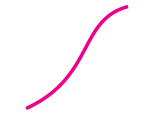
\includegraphics[width=.8in]{12-09P}
        \end{center}
        Which of the following statements \textbf{best} matches the company's performance?
        \begin{enumerate}[(i)]
        \item We're losing money, and it's getting worse as time goes on.
        \item The outlook is great: The growth rate keeps increasing.
        \item We're doing well, but our growth rate is leveling off.
        \item We're losing money, but not as quickly as before.
        \item Business had been picking up, but now it's cooling off.
        \item Business had been cooling off, but now it's picking up.
        \end{enumerate}
\end{problem}


\begin{problem}
        Sketch the graph of a function $f(x)$ with $f(0) = 0$ that has the given sign charts for $f'(x)$ and $f''(x)$.
        \begin{center}
                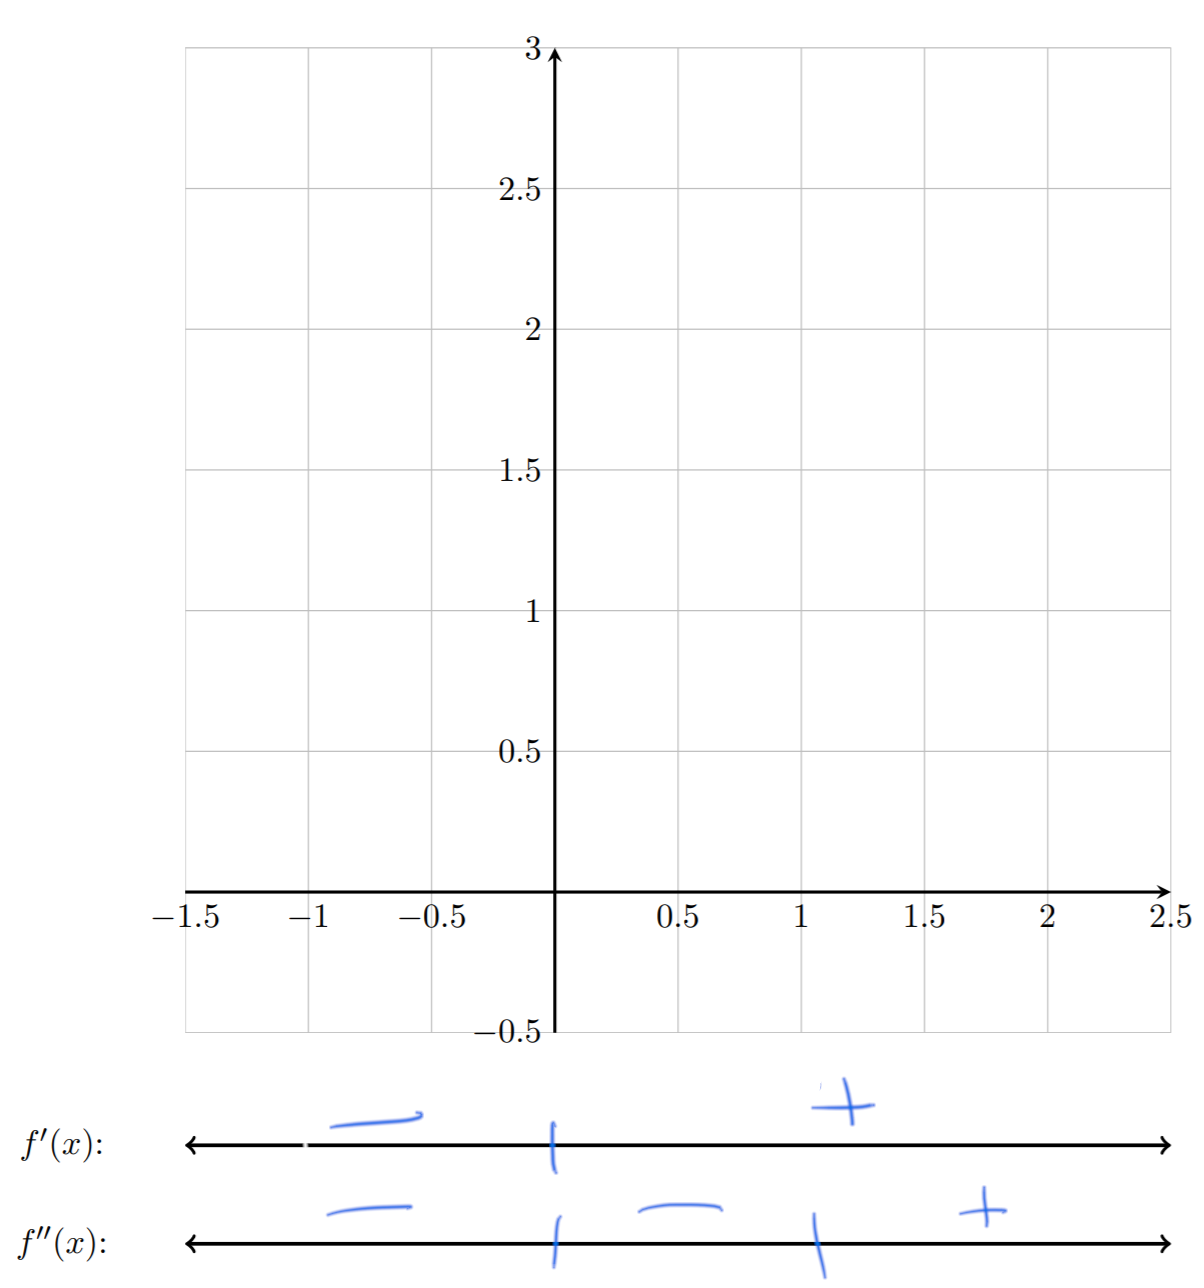
\includegraphics[width=.9\textwidth]{12-09P2}
        \end{center}
\end{problem}
\end{document}



